\chapter{Clean Code Development Grundlagen}
\section{Womit beschäftigt sich CCD?}
\SuperPar Wie in der Einleitung bereits erläutert beschäftigt sich CCD in erster Linie mit dem Schreiben von lesbaren Code. Es sollte dabei bei der Implementierung geachtet werden, dass
In der Abbildung \ref{fig:cycle} ist ein Kreislauf dargestellt, der die drei Hauptpunkte darstellt und auch zeigt, dass diese sich gegenseitig beeinflussen. Durch die gute Lesbarkeit, wird die Wartbarkeit des Codes erhöht. Da sich selbst ein neuer Mitarbeiter schnell einlesen kann und gut erkennen kann welche Aufgabe der aktuell betrachtete Code hat sind die Einarbeitungszeiten für Mitarbeiter außerdem viel kürzer. Durch die bessere Wartbarkeit ergibt sich im weiteren auch die besseren Testbarkeit, welche für die Qualität der Software von hoher Bedeutung ist, da nur für getesteten Code sichergestellt werden kann, dass dieser auch wirklich die gewünschte Aufgabe richtig erledigt. Diese verbesserte Testbarkeit führt schließlich zu einer besseren Lesbarkeit, da die Test mit einer Dokumentation des Codes verglichen werden können. Sie zeigen welche Ausgabe erwartet werden kann und meist zeigen diese Tests auch Grenzfälle.

\begin{figure}[h]
	\centering
		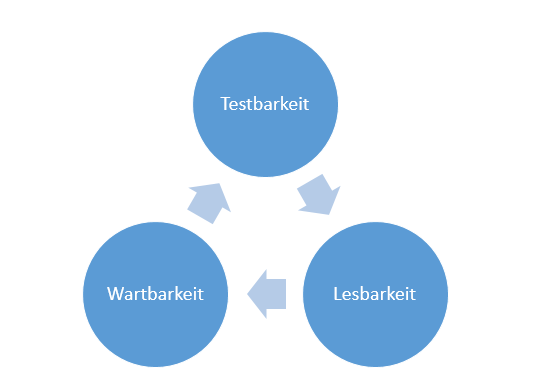
\includegraphics[width=1.00\textwidth]{images/cycle.PNG}
	\caption{CCD Zyklus}
	\label{fig:cycle}
\end{figure}

\section{Ziele von CCD}
\SuperPar Die wichtigsten Ziele von CCD sind es, den Quellcode 

\section{Die Pfadfinder-Regel}
\SuperPar Eine der grundlegendsten Regeln im CCD ist die sogenannte Pfadfinder-Regel. Robert C. Martin definiert diese in \cite{CleanCode} wie folgt:

\begin{quote}
	Hinterlasse den Campingplatz sauberer, als du ihn gefunden hast.
\end{quote}

\SuperPar Auf die Arbeit eines Programmierers oder einer Programmiererin umgemünzt bedeutet dieser Leitsatz, dass jede Klasse, welche man auscheckt oder betrachtet verbessert werden sollte. Dies muss nicht immer ein großes Refactoring oder ein verbessern der Gesamtstruktur sein. Es reicht meist schon, für eine Variable einen besseren Namen zu vergeben, oder einen unnötigen Kommentar zu entfernen. Robert C. Martin schreibt weiters, dass sich durch dieses vorgehen ein für die Softwareentwicklung ungewöhnlicher Trend ergibt. Der Quelltext wird über die Zeit besser. Er verbindet dieses Verhalten außerdem mit professionelem Verhalten. Ein professioneller, verantwortungsbewusster Programmierer versucht ständig, die Codebasis zu verbessern.

\section{Smells und Heuristiken}
\SuperPar Robert C. Martin beschreibt in \cite{CleanCode} eine Liste von Smells und Heuristken, welche Probleme beschreiben, die sehr häufige Ursachen für schlechten Code darstellen.
\subsection{Kommentare}

\begin{table}[h]
	\centering
		 \begin{tabular}{ | l | }
		 \hline
			Name \\  \hline
			Ungeeignete Informationen\\
			Überholte Kommentare  \\
			Redundante Kommentare \\
			Schlecht geschriebene Kommentare  \\
			Auskommentierter Code \\ \hline
		\end{tabular}
	\caption{Smells und Heuristiken für Kommentare}
	\label{tab:SmellsUndHeuristiken_Comments}
\end{table}

\subsection{Umgebung}

\begin{table}[h]
	\centering
		 \begin{tabular}{ | l | }
		 \hline
			Name \\  \hline
			Ein Build erfordert mehr als einen Schritt \\
			Test erfordern mehr als einen Schritt \\ \hline
		\end{tabular}
	\caption{Smells und Heuristiken für die Umgebung}
	\label{tab:SmellsUndHeuristiken_Umgebung}
\end{table}

\subsection{Funktionen}

\begin{table}[h]
	\centering
		 \begin{tabular}{ | l | }
		 \hline
			Name \\  \hline
			Zu viele Argumente \\
			Output-Argumente \\
			Flag-Argumente \\
			Tote Funktionen \\ \hline
		\end{tabular}
	\caption{Smells und Heuristiken für Funktionen}
	\label{tab:SmellsUndHeuristiken_Functions}
\end{table}

\subsection{Allgemein}

\begin{table}[h]
	\centering
		 \begin{tabular}{ | l | }
		 \hline
			Name \\  \hline
			Mehrere Sprachen in einer Quelldatei \\
			Offensichtliches Verhalten ist nicht implementiert \\
			Falsches Verhalten an den Grenzen \\
			Übergangene Sicherungen \\
			Duplizierung \\
			Auf der falschen Abstraktionsebene codieren \\
			Basisklasse hängt von abgeleiteten Klassen ab \\
			Zu viele Informationen \\
			Toter Code \\
			Vertikale Trennung \\
			Inkonsistenz \\
			Müll \\
			Künstliche Kopplung \\
			Funktionsneid \\
			Selektor-Argumente \\
			Verdeckte Absicht \\
			Falsche Zuständigkeit \\
			Fälschlich als statisch deklarierte Methode \\
			Aussagekräftige Variablen verwenden \\
			Funktionsname sollte die Aktion ausdrücken \\
			Den Algorithmus verstehen \\
			Logische Abhängikeiten in phyische umwandeln \\
			Polymorphismus statt If/Else oder Switch/Case verwenden \\
			Konventionen beachten \\
			Magische Zahlen durch benannte Konstanten ersetzen \\
			Präzise sein \\
			Struktur ist wichtiger als Konvention \\
			Bedingungen einkapseln \\
			Negative Bedingungen vermeiden \\
			Eine Aufgabe pro Funktion! \\
			Verborgene zeitliche Kopplungen \\
			Keine Willkür \\
			Grenzbedingungen einkapseln \\
			In Funktionen nur eine Abstraktionsebene tiefer gehen \\
			Konfigurierbare Daten hoch ansiedeln \\
			Transitive Navigation vermeiden \\ \hline
		\end{tabular}
	\caption{Smells und Heuristiken für Kommentare}
	\label{tab:SmellsUndHeuristiken_Comments}
\end{table}

\subsection{Namen}

\begin{table}[h]
	\centering
		 \begin{tabular}{ | l | }
		 \hline
			Name \\  \hline
			Deskriptive Namen wählen \\
			Namen sollten der Abstraktionsebene entsprechen \\
			Möglichst die Standardnomenklatur verwenden \\
			Eindeutige Namen \\
			Lange Namen für große Geltungsbereiche \\
			Codierungen vermeiden \\
			Namen sollten Nebeneffekte beschreiben \\ \hline
		\end{tabular}
	\caption{Smells und Heuristiken für die Umgebung}
	\label{tab:SmellsUndHeuristiken_Umgebung}
\end{table}


\subsection{Tests}

\begin{table}[h]
	\centering
		 \begin{tabular}{ | l | }
		 \hline
			Name \\  \hline
			Unzureichende Tests \\
			Ein Coverage-Tool verwenden \\
			Triviale Tests nicht überspringen \\
			Ein ignorierter Test zeigt eine Mehrdeutigkeit auf \\
			Grenzbedingungen testen \\
			Bei Bugs die Nachbarschaft gründlich testen \\
			Das Muster des Scheiterns zur Diagnose nutzen \\
			Hinweise druch Coverage-Patterns \\
			Testen sollten schnell sein \\ \hline
		\end{tabular}
	\caption{Smells und Heuristiken für die Umgebung}
	\label{tab:SmellsUndHeuristiken_Umgebung}
\end{table}

\section{Coding Conventions}
\label{cha:CodingConventions}
Coding Conventions sind ein sehr effizientes Mittel projektweite, oder auch unternehmensweite Regeln zu definieren, wie einzelne Aspekte der Programmierung gestaltet werden sollten. Vor allem für Opensource Projekte ist dies ein sehr wichtiges Mittel wie ein durchgängiger Codierungsstil gewählt werden kann. Meist werden auch für Frameworks Coding Conventions definiert wie zum Beispiel für C\# \cite{CSHARPCoding}. Meist werden diese grundlegenden Konventionen von Unternehmen verwendet und nur teilweise angepasst, da es durch einen durchgängigen Programmierstil für eine Plattform leichter ist, dass sich neue Programmierer oder Programmiererinnen in die Codebasis einarbeiten. Ein wichtiger Aspekt der bei Coding Conventions beachtet werden muss, ist die Möglichkeit der automatischen Überprüfung dieser. Dazu werden in Abschnitt \ref{cha:CheckingCCDCriterias} einige Möglichkeiten erläutert, wie die Überprüfung dieser Kriterien erfolgen kann.

 
\section{Überprüfung der CCD Kriterien}
\label{cha:CheckingCCDCriterias}
\SuperPar Häufig stellt sich beim CCD die Frage, wie es möglich ist die einzelnen Kriterien zu überprüfen. Hierzu gibt es verschiedene Varianten. Es gibt einerseits die statische Codeanalyse, welche dafür Sorgen kann, dass die in Abschnitt \ref{cha:CodingConventions} beschriebenen Coding Conventions eingehalten werden. Ein sehr wirksames Mittel für die Überprüfung des Quellcodes allgemein sind Coding Reviews. Es sollte in den folgenden Abschnitten näher auf diese beiden Werkzeuge eingegangen werden.

\subsection{Statische Codeanalyse}
\SuperPar Die statische Codeanalyse bietet eine Möglichkeit zur Analyse des Quellcodes nach fix vorgegebenen Regeln. Dabei werden für ein Unternehmen, oder für ein Projekt die Abschnitt \ref{cha:CodingConventions} beschriebenen Coding Conventions festegelegt und an Hand dieser Regeln definiert. Ein Beispiel für solch eine Regel wäre das in C\# übliche \textit{I} vor einem Interfacenamen. Das Tool für die statische Codeanalyse würde im Falle einer Missachtung dieser Regel eine Warnung ausgeben und der Programmierer würde direkt darauf aufmerksam gemacht werden, dass er sich nicht an die Coding Conventions hält. Im .NET Bereich ist das wohl bekannteste statische Codeanalyse Tool NDepend (http://www.ndepend.com/). Mit diesem ist es neben den überprüfen der Coding Conventions auch möglich, zirkuläre Abhängigkeiten zwischen Klassen zu erkennen, zyklische Komplexitäten von Methoden zu analysieren und viele weitere Metriken zu erzeugen, die Aufschluss darüber geben, wie sauber der analysierte Code programmiert wurde. Im Java Bereich gibt es das sehr hilfreiche Tool JDepend (http://clarkware.com/software/JDepend.html) welches ähnlich aufgebaut ist wie NDepend.

\subsection{Code Reviews}
\SuperPar Code Reviews sind ein sehr wirksames Mittel um geschriebenen Code zu Überprüfen. Es handelt sich bei diesen Reviews um manuelle Überprüfungen, die meist von erfahreneren Entwicklern vorgenommen werden. Dabei ist einer der wichtigsten Punkte, dass das Review nicht durch die Person erfolgt, die den Quellcode produziert hat, sondern durch jemand anderen. Weiters gibt es die Möglichkeit ein sogenanntes Peer Review durchzuführen. Bei diesem führen die Person, die den Quellcode produziert hat und eine zweite Person das Review durch und besprechen den vorliegenden Code. An dieser Stelle sollte das Prinzip des Pair Programmings, das aus dem Extreme Programming kommt erwähnt werden. \cite{BeckExtreme} 